%%%%%%%%%%%%%%%%%%%%%%%%%%%%%%%%%%%%%%%%%%%%%%%%%%%%%%%%%%%%%%%%%%%%%%
% Problem statement
\begin{statement}[
  problempoints=110,
  timelimit=1 second,
  memorylimit=512 MiB,
]{Drvca}

\setlength\intextsep{-0.1cm}
\begin{wrapfigure}[8]{r}{0.25\textwidth}
\centering
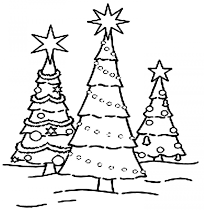
\includegraphics[width=0.25\textwidth]{img/drvca.png}
\end{wrapfigure}

\textit{Advent in Zagreb} is a traditional holiday manifestation whose main
attraction is a magical Christmas market located at the city centre. It
should also be noted that this event was voted the best in Europe for three
years in a row. Apart from travelling fast, good news also has the tendency
to travel far. Indeed, the information about Advent in Zagreb reached North
Pole and Santa Claus himself. Interestingly enough, Santa never visited
Croatia (except for usual business on Christmas Eve). When you think about
it, that makes sense since he doesn't really like summer activities by the
sea and he can solve COCI problems from the comfort of his own home.

Luckily, he decided to visit our Christmas market so he sent a letter to the
town hall stating that he will land on Zagreb's main square in the early morning
of December 14\textsuperscript{th}. After his on-site participation in a COCI round, he
will have a guided tour of Zagreb's finest gastronomic sites by Mr. Malnar.

You are probably wondering: ``How exactly does Santa plan to land, there is no
runway there!''. You are right, there is not, but we'll manage. The town hall
already prepared $N$ Christmas trees that should be featured on the main square.
Now, they will simply take those trees and place them in two rows which will
define the boundaries of the runway. For some reason they want to make the
absolute difference in height between each two neighbouring trees to be the
same in each row. Moreover, they want to have the trees sorted in each row from
the shortest to the highest. Help them divide the trees into two rows that
satisfy these conditions.

%%%%%%%%%%%%%%%%%%%%%%%%%%%%%%%%%%%%%%%%%%%%%%%%%%%%%%%%%%%%%%%%%%%%%%
% Input
\subsection*{Input}
The first line contains an integer $N$ $(2 \le N \le 10^5)$ from the task
description.

The next line contains $N$ integers $h_i$ $(1 \le h_i \le 10^9)$ that denote
the heights of all $N$ Christmas trees.

%%%%%%%%%%%%%%%%%%%%%%%%%%%%%%%%%%%%%%%%%%%%%%%%%%%%%%%%%%%%%%%%%%%%%%
% Output
\subsection*{Output}
In the first line you should output an integer $A$ which represents the number
of trees in the first row. In the second line you should output $A$ integers
which represent the heights of the trees in the first row of the runway.

In the third line you should output an integer $B$ which represents the number
of trees in the second row. In the fourth line you should output $B$ integers
which represent the heights of the trees in the second row of the runway.

The rows are not allowed to be empty $(A > 0$ and $B > 0)$ and each tree should
be a part of one row $(A + B = N)$. Also, trees should be sorted in each row
from the shortest to the highest. If there are multiple solutions, you can
output any of them. If there is no solution which satisfies the necessary
conditions, you should output $-1$ in the only line of output.

%%%%%%%%%%%%%%%%%%%%%%%%%%%%%%%%%%%%%%%%%%%%%%%%%%%%%%%%%%%%%%%%%%%%%%
% Scoring
 \subsection*{Scoring}
{\renewcommand{\arraystretch}{1.4}
  \setlength{\tabcolsep}{6pt}
  \begin{tabular}{ccl}
 Subtask & Score & Constraints \\ \midrule
  1 & 20 & $N \le 15$ \\
  2 & 30 & $N \le 300$ \\
  3 & 30 & \makecell[l]{$N \le 10^5$,
            there is a solution in which both rows have the same number of trees.
            } \\
  4 & 30 & No additional constraints. \\
\end{tabular}}

%%%%%%%%%%%%%%%%%%%%%%%%%%%%%%%%%%%%%%%%%%%%%%%%%%%%%%%%%%%%%%%%%%%%%%
% Examples
\subsection*{Examples}
\begin{tabularx}{\textwidth}{X'X'X}
\sampleinputs{test/drvca.dummy.in.1}{test/drvca.dummy.out.1} &
\sampleinputs{test/drvca.dummy.in.2}{test/drvca.dummy.out.2} &
\sampleinputs{test/drvca.dummy.in.3}{test/drvca.dummy.out.3}
\end{tabularx}

%%%%%%%%%%%%%%%%%%%%%%%%%%%%%%%%%%%%%%%%%%%%%%%%%%%%%%%%%%%%%%%%%%%%%%
% We're done
\end{statement}

%%% Local Variables:
%%% mode: latex
%%% mode: flyspell
%%% ispell-local-dictionary: "croatian"
%%% TeX-master: "../hio.tex"
%%% End:
